\documentclass[border=2mm]{standalone}


\usepackage{pgfplots}
\pgfplotsset{compat=1.18}
\usetikzlibrary{arrows.meta, calc, positioning, decorations.pathreplacing, calligraphy}

\usepackage{xcolor}
\definecolor{den-1}{HTML}{111111}   % Đen #111111
\definecolor{den-2}{HTML}{222222}   % Đen #222222
\definecolor{den-3}{HTML}{333333}   % Đen #333333
\definecolor{den-4}{HTML}{444444}   % Đen #444444
\definecolor{den-5}{HTML}{555555}   % Đen #555555
\definecolor{den-6}{HTML}{666666}   % Đen #666666

\tikzset{
  >=Stealth,
  originlabel/.style={
    font=\small\sf,
    anchor=north east, 
    yshift=-0.1ex,     
    xshift=-0.1ex      
  }
}

\begin{document}

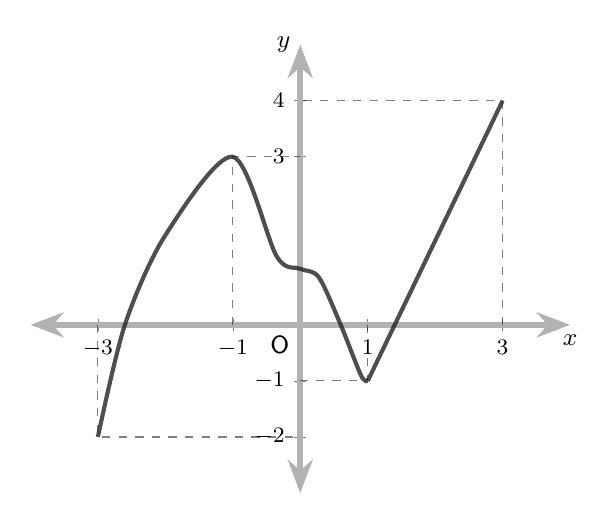
\begin{tikzpicture}

  \begin{axis}[
    font=\small\sf,
    axis lines=middle,
    axis line style={<->, line width=2pt, color=den-6!50},
    xlabel=$x$, ylabel=$y$,
    xlabel style={below, font=\small\sf},
    ylabel style={left, font=\small\sf},
    ymin = -3, ymax = 5,
    xmin = -4, xmax = 4,
    xtick = {-3, -1, 0, 1, 3},
    ytick = {-2, -1, 0, 3, 4},
    tick label style={font=\footnotesize\sf},
    clip=false,
  ]

  \node[originlabel] at (axis cs:0,0) {O};

  \draw [dashed, opacity=.5] (-3,0) -- (-3,-2) -- (0,-2);
  \draw [dashed, opacity=.5] (-1,0) -- (-1,3) -- (0,3);
  \draw [dashed, opacity=.5] (1,0) -- (1,-1) -- (0,-1);
  \draw [dashed, opacity=.5] (3,0) -- (3,4) -- (0,4);

  \addplot[
    smooth,
    line width=1.5pt,
    color=den-2,
    opacity=.8
  ] coordinates {
    (-3, -2)
    (-2.6,0)
    (-2,1.6)
    (-1, 3)
    (-.35,1.225)   
    (0, 1)
    (.275,.85)
    (.6,0)
    (.9,-.9)
    (1, -1)
  };
  
  \addplot[
    smooth,
    line width=1.5pt,
    color=den-2,
    opacity=.8
  ] coordinates {
    (1, -1)
    (3, 4)
  };

    

  \end{axis}
\end{tikzpicture}
\end{document}
